
\newcommand{\ttf}[1]{\texttt{#1}\xspace}
\newcommand{\dpc}{\ttf{D-2PC}}
\newcommand{\cpc}{\ttf{C-2PC}}

\chapter{Coordination: Concepts and Costs}
\label{c.background}

In this chapter, we further examine the concept of coordination and
why we seek to avoid it. We discuss traditional uses of coordination
to maintain correct data in database systems and measure its costs in
modern distributed environment, which we will attempt to circumvent in
the remainder of this thesis. We also present our formal system model
for replicated databases.

\section{Coordination and Correctness in Database Systems}
\label{sec:t-motivation}
As repositories for application state, databases are traditionally
tasked with maintaining, informally, ``correct'' data---that is, data
that obey some semantic guarantees about their integrity---on behalf
of users. Thus, during concurrent access to data, a database ensuring
data correctness must therefore decide which user operations can
execute simultaneously and which, if any, cannot. Informally, we say
that two operations within a database must \textit{coordinate} if they
cannot execute concurrently on independent copies of the database state
(Section~\ref{sec:model} provides a more formal treatment).

\minihead{By example} Consider a database-backed payroll application
that maintains information about employees and departments within a
small business. In the application, $a.)$ each employee is assigned a
unique ID number and $b.)$ each employee belongs to exactly one
department. A database ensuring correctness must maintain these
application-level semantic guarantees (or data \textit{invariants}) on
behalf of the application (i.e., without application-level
intervention). In our payroll application, this is non-trivial: for
example, if the application attempts to simultaneously create two
employees by examining the set of currently assigned IDs and choosing
an unassigned ID for each new employee, then the database must ensure
the employees are assigned distinct IDs.

\minihead{Serializability and conflicts} The classic answer to
maintaining application-level invariants is to use serializable
isolation: execute each user's ordered sequence of operations, or
\textit{transactions}, such that the end result is equivalent to some
sequential execution~\cite{tamer-book,bernstein-book,gray-virtues}. If
each transaction preserves correctness in isolation, composition via
serializable execution ensures correctness. In our payroll example,
the database would execute the two employee creation transactions such
that one transaction appears to execute after the other. The second
transaction would observe the ID that the first transaction chose,
thus avoiding duplicate ID assignment.

While serializability is a powerful abstraction, it comes with a cost:
for arbitrary transactions (and for all implementations of
serializability's more conservative variant---conflict
serializability), any two operations to the same item---at least one
of which is a write---will result in a \textit{read/write
  conflict}. Under serializability, these conflicts require
coordination: to provide a serial ordering, conflicts must be totally
ordered across transactions, and so transactions cannot proceed
entirely independently~\cite{bernstein-book}. As a canonical example,
given initial database state containing two variables $x$ and $y$,
where $\{x=\bot, y=\bot\}$, if transaction $T_1$ reads from $y$ and
writes $x=1$ and and $T_2$ reads from $x$ and writes $y=1$, then a
database cannot both execute $T_1$ and $T_2$ independently on separate
copies of state while maintaining
serializability~\cite{davidson-survey,hat-vldb}.\footnote{This
  read-write pattern might arise in our ID assignment scenario: $T_1$
  attempts to reserve ID $1$ for its user, $x$, while $T_2$ attempts
  to reserve ID $1$ for its user, $y$. If the two transactions run
  concurrently on separate copies of the database, neither $T_1$ nor
  $T_2$ would observe the others's updates. We present this example in
  terms of reads and writes because it is standard and to highlight
  the fact that serializability enforces concurrency by examining
  read/write access to variables, not by examining the program
  semantics.}

Because serializable semantics require coordination, \textit{all}
database implementations that provide serializability will
coordinate. For example, a database could use two-phase
locking~\cite{gray-isolation} to provide serializability: in a
simplified protocol, the first time a transaction accesses a data
item $x$, the transaction can acquire an exclusive lock on $x$; once
the transaction has completed all of its operations on the database,
it can release all of its locks. In this protocol, locks form a point
of coordination between concurrent transactions: while one transaction
holds an exclusive lock on an item, other transactions that wish to
operate on the same item cannot make progress.

\minihead{Semantics, Sufficiency, and Necessity} It is often
convenient to reason about semantic guarantees instead of concrete
implementations of those guarantees. Instead of examining concurrency
control mechanisms one-by-one (e.g., multi-version concurrency
control, optimistic concurrency control, pre-scheduling, and so on),
we can unequivocally determine---as in the case of
serializability---that all implementations of a given semantics
require coordination to enforce.

However, the converse does not hold: just because a given
implementation of a guarantee uses coordination does not mean that the
guarantee necessarily requires coordination for enforcement. For
example, even though a database may employ serializability to enforce
an invariant, the invariant may not \textit{require} coordination for
correct enforcement. There may or may not be ways to enforce the
invariants without coordination. In general, we can always
coordinate. The core question is whether coordination is necessary for
a given invariant or semantic property.

\section{Understanding the Costs of Coordination}

Why worry about coordination? Peter Deutsch starts his classic list of
``Fallacies of Distributed Computing'' with two concerns fundamental
to distributed database systems: ``\textit{1.)}  The network is
reliable. \textit{2.)} Latency is zero''~\cite{fallacies-deutsch}. In
a distributed setting, network failures may prevent database servers
from communicating, and, in the absence of failures, communication is
slowed by factors like physical distance, network congestion, and
routing. Thus, as we discuss here, the costs of coordination can be
observed across three primary dimensions: increased latency, decreased
throughput, and, in the event of partial failures, unavailability. In
this section, we examine these costs in detail.


\subsection{Latency}
\label{sec:latency}

Even with fault-free networks, distributed systems face the challenge
of network communication latency. If two operations running on two
separate servers must coordinate, then the latency experienced by the
operations will be bounded from below by the amount of time required to
exchange information between the sites. In this section, we quantify
network latencies of modern cloud computing environments. These are
often large and may exceed hundreds of milliseconds in a
geo-replicated, multi-datacenter context.  Fundamentally, the speed at
which two servers can communicate is (according to modern physics)
bounded by the speed of light. In the best case, two servers on
opposite sides of the Earth communicating via a hypothetical link
through the planet's core would require a minimum 85.1~ms round-trip
time (RTT; 133.7~ms if sent at surface level). As services are
replicated to multiple, geographically distinct sites, the cost of
communication between replicas increases.

\definecolor{min-lat-color}{HTML}{B2FF99}
\definecolor{max-lat-color}{HTML}{FF7F7F}

\begin{table}[t!]

\subfloat[Within \texttt{us-east-b} availability zone] {
  \makebox[.5\textwidth]{
 \begin{tabular}{|c|c|c|}\hline
 & \multicolumn{1}{c}{H2} & \multicolumn{1}{c|}{H3}\\\hline
H1  & 0.55   & \colorbox{max-lat-color}{0.56} \\
H2 &  & \colorbox{min-lat-color}{0.50}  \\
\hline
  \end{tabular}}
 }
\subfloat[Across \texttt{us-east} availability zones]{
  \makebox[.5\textwidth]{
    \begin{tabular}{|c|c|c|}\hline
 & \multicolumn{1}{c}{C} & \multicolumn{1}{c|}{D}\\\hline
B & \colorbox{min-lat-color}{1.08} & 3.12 \\
C & & \colorbox{max-lat-color}{3.57}  \\
\hline
  \end{tabular}}
}\vspace{.5em}

\subfloat[Cross-region (CA:~California, OR:~Oregon, VA:~Virginia, TO:~Tokyo, IR:~Ireland, SY:~Sydney, SP:~S\~{a}o Paulo, SI:~Singapore)] {
  \begin{tabular}{|c|c|c|c|c|c|c|c|c|}
\hline
& \multicolumn{1}{c}{OR} & \multicolumn{1}{c}{VA} & \multicolumn{1}{c}{TO} & \multicolumn{1}{c}{IR} & \multicolumn{1}{c}{SY} & \multicolumn{1}{c}{SP} & \multicolumn{1}{c|}{SI} \\\hline
CA & \colorbox{min-lat-color}{22.5}   & 84.5   & 143.7   & 169.8   & 179.1   & 185.9   & 186.9  \\
OR &  & 82.9   & 135.1   & 170.6   & 200.6   & 207.8   & 234.4  \\
VA & &  & 202.4   & 107.9   & 265.6   & 163.4   & 253.5  \\
TO & & &  & 278.3   & 144.2   & 301.4   & 90.6  \\
IR & & & &  & 346.2   & 239.8   & 234.1  \\
SY & & & & &  & 333.6   & 243.1  \\
SP & & & & & &  & \colorbox{max-lat-color}{362.8}  \\
\hline
  \end{tabular}\vspace{.5em}
}\vspace{1em}

\caption{Mean RTT times on EC2 (min and max highlighted)}
\label{table:rtt}
\end{table}

\begin{figure}[t!]
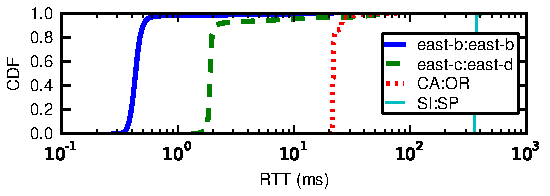
\includegraphics[width=\figscale\columnwidth]{figs/ping-plot.pdf}\vspace{.5em}
\caption{CDF of round-trip times for slowest inter- and intra-
  availability zone links compared to cross-region links.}
\label{fig:rtt}
\end{figure}

In actual server deployments, messages travel slower than the speed of
light due to routing, congestion, and computational overheads. To
illustrate the behavior of intra-datacenter, inter-datacenter, and
inter-planetary networks, we performed a measurement study of network
behavior on Amazon's Elastic Compute Cloud (EC2), a widely used public
compute cloud. We measured one week of ping times (i.e., round-trip
times, or RTTs) between all seven EC2 geographic ``regions,'' across
three ``availability zones'' (closely co-located datacenters), and
within a single ``availability zone'' (datacenter), at a granularity
of 1s. We summarize the results of our network measurement study in
Table~\ref{table:rtt}. On average, intra-datacenter communication
(Table~\ref{table:rtt}a) is between 1.82 and 6.38 times faster than
across geographically co-located datacenters (Table~\ref{table:rtt}b)
and between 40 and 647 times faster than across geographically
distributed datacenters (Table~\ref{table:rtt}c). The cost of
wide-area communication exceeds the speed of light: for example, while
a speed-of-light RTT from S\~{a}o Paulo to Singapore RTT is 106.7~ms,
ping packets incur an average 362.8~ms RTT (95th percentile: 649~ms). As
shown in Figure~\ref{fig:rtt}, the distribution of latencies varies
between links, but the overall trend is clear: coordination may lead
to substantial delays. Quantifying and minimizing communication delays
is also an active area of research in the networking
community~\cite{bobtail}.

\subsection{Throughput and Scalability}
\label{sec:background-cmotivation}

Coordination also affects throughput. If a transaction takes $d$
seconds to execute, the maximum throughput of coordinating
transactions operating on the same items under a general-purpose
(i.e., interactive, non-batched) transaction model is limited by
$\frac{1}{d}$. Any operations that arrive in excess of this limit will
also have to wait. Within a single server, delays can be small,
permitting tens to hundreds of thousands of conflicting transactions
per item per second. In a partitioned database system, where different
items are located on different servers, or in a replicated database
system, where the same item is located (and is available for
operations) on multiple servers, the cost increases: delay is
lower-bounded by network latency. On a local area network, delay may
vary from several microseconds (e.g., via Infiniband or RDMA) to
several milliseconds on today's cloud infrastructure, permitting
anywhere from a few hundred transactions to a few hundred thousand
transactions per second. However, as we have seen, a wide-area
network, delay is lower-bounded by the speed of light (worst-case on
Earth, around 75~ms, or about 13 operations per
second~\cite{hat-vldb}). Under network
partitions~\cite{queue-partitions}, as delay tends towards infinity,
these penalties lead to unavailability~\cite{gilbert-cap,hat-vldb}. In
contrast, operations executing without coordination can proceed
concurrently and will not incur these penalties.

To further understand the costs of coordination, we performed two sets
of measurements---one using a database prototype and one using traces
from prior studies.  We first compared the throughput of a set of
coordinated and coordination-free transaction execution. Our basic
workload is simple: a set of transactions read and increment a set of
integers stored on separate servers.


First, we implemented two coordinated algorithms: traditional
two-phase locking and an optimized variant of two-phase locking, both
on in-memory data. In two-phase locking, each client acquires locks
one at a time, requiring a full round trip time (RTT) for every lock
request. For an $N$ item transaction, locks are held for $2N+1$
message delays (the $+1$ is due to broadcasting the unlock/commit
command to the participating servers). Our optimized two-phase locking
only uses one message delay (half RTT) to perform each lock request:
the client specifies the entire set of items it wishes to modify at
the start of the transaction (in our implementation, the number of
items in the transaction and the starting item ID), and, once a server
has updated its respective item, the server forwards the remainder of
the transaction to the server responsible for the next write in the
transaction (similar to linear commit
protocols~\cite{bernstein-book}). For an $N$-item transaction, locks
are only held for $N$ message delays (the final server both broadcasts
the unlock request to all other servers and also notifies the client),
while a $1$-item transaction does not require distributed locking.

To avoid deadlock (which we found was otherwise common in this
high-contention microbenchmark), our implementation totally orders any
lock requests according to item and executes them sequentially (e.g.,
lock item $1$ then lock item $2$ and so on). Our implementation also
piggybacks operation commands along with lock requests, further
avoiding message delays. Since we are only locking one item per
server, our microbenchmark code does not use a dynamic lock manager
and instead associates a single lock with each item; this further
lowers locking overheads.

Our coordination-free transaction implementation is simpler: it uses
no locks and simply performs the increment operation across each
transaction in parallel, without acquiring locks.

We partitioned eight in-memory items (integers) across eight
\texttt{cr1.8xlarge} Amazon EC2 instances with clients located on a
separate set of \texttt{cr1.8xlarge}
instances. Figure~\ref{fig:micro-all} reported in depicts results for
the coordination-free implementation and the optimized two-phase
locking case. Unsurprisingly, two-phase locking performs worse than
optimized two-phase locking, but both incur substantial penalties due
to coordination delay over the network.

\begin{figure}
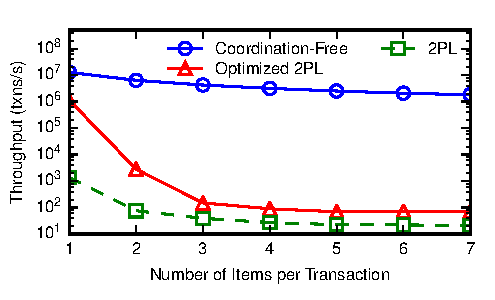
\includegraphics[width=\figscale\columnwidth]{figs/micro_thru_all.pdf}
\caption{Microbenchmark performance of coordinated and
  coordination-free execution of transactions of varying size writing
  to eight items located on eight separate multi-core servers.}
\label{fig:micro-all}
\end{figure}

With single-item, non-distributed transactions, the coordination-free
implementation achieves, in aggregate, over 12M transactions per
second and bottlenecks on \textit{physical resources}---namely, CPU
cycles. In contrast, the lock-based implementation achieves
approximately $1.1$M transactions per second: it is unable to fully
utilize all 32 multi-core processor contexts due to lock contention. For
distributed transactions, coordination-free throughput decreases
linearly (as an $N$-item transaction performs $N$ writes), while the
throughput of coordinating transactions drops by over three orders of
magnitude.

While the above microbenchmark demonstrates the costs of a particular
\textit{implementation} of coordination, we also studied the
effect of more fundamental, implementation-independent overheads
(i.e., also applicable to optimistic and scheduling-based concurrency
control mechanisms). We determined the maximum attainable throughput
for coordinated execution within a single datacenter (based on data
from~\cite{bobtail}) and across multiple datacenters (based on data
from~\cite{hat-vldb}) due to blocking coordination during atomic
commitment~\cite{bernstein-book}. 

We simulate traditional two-phase commit~\cite{bernstein-book} and
decentralized two-phase commit~\cite{paxos-commit} using network
models derived from existing studies. For an $N$-server transaction,
classic two-phase commit (\cpc) requires $N$ (parallel) coordinator to
server RTTs, while decentralized two-phase commit (\dpc) requires $N$
(parallel) server to server broadcasts, or $N^2$ messages. Our
simulation is straightforward, but we make several
optimizations to improve the throughput of each algorithm. First, we
assume that transactions are pipelined, so that each server can
\texttt{prepare} immediately after it has \texttt{commit}ted the prior
transaction. Second, our pipelines are ideal in that we do not
consider deadlock: only one transaction \texttt{prepare}s at a given
time. Third, we do not consider the cost of local processing of each
transaction: throughput is determined entirely by communication delay.

Figure~\ref{fig:2pc} shows that, in the local area, with only two
servers (e.g., two replicas or two coordinating operations on items
residing on different servers), throughput is bounded by 1125
transactions per second (via \dpc; 668 transactions per second via
\cpc). Across eight servers, \dpc throughput drops to 173 transactions
per second (respectively 321 for \cpc) due to long-tailed latency
distributions. In the wide area, the effects are more severe: if
coordinating from Virginia to Oregon, \dpc message delays are 83~ms
per commit, allowing 12 operations per second. If coordinating between
all eight EC2 availability zones, throughput drops to slightly over 2
transactions per second in both algorithms.

These results should also be unsurprising: coordinating---especially over
the network---can incur serious throughput penalties. In contrast,
coordination-free operations can execute without incurring these
costs. The costs of actual workloads can vary: if coordinating
operations are rare, concurrency control will not be a bottleneck. For
example, a serializable database executing transactions with disjoint
read and write sets can perform as well as a non-serializable database
without compromising correctness~\cite{shore-communication}. However,
as these results demonstrate, minimizing the amount of coordination
and its degree of distribution can therefore have a tangible impact on
performance, latency, and
availability~\cite{pacelc,hat-vldb,gilbert-cap}. While we study real
applications in Section~\ref{sec:evaluation}, these measurements
highlight the worst of coordination costs on modern hardware.

\begin{figure}
  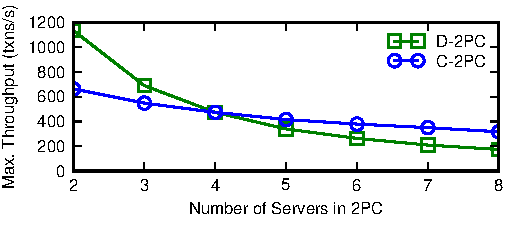
\includegraphics[width=.8\columnwidth]{figs/singledc-twopc.pdf}\\
  {\centering {\small a.) Maximum serializable transaction
      throughput over local-area network in~\cite{bobtail}}\par}
  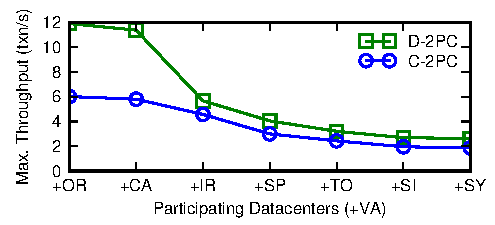
\includegraphics[width=.8\columnwidth]{figs/multidc-twopc.pdf}\\
  {\small b.) Maximum serializable transaction throughput
    over wide-area network in~\cite{hat-vldb} with transactions
    originating from a coordinator in Virginia (VA; OR:~Oregon,
    CA:~California, IR:~Ireland, SP:~S\~{a}o Paulo, TO:~Tokyo,
    SI:~Singapore, SY:~Sydney)}\vspace{1em}

  \caption{Atomic commitment latency as an upper bound on conflicting
    serializable transaction throughput over local-area and wide-area networks.}
\label{fig:2pc}
\end{figure}

While this study is based solely on reported latencies, deployment
reports corroborate our findings. For example, Google's F1 uses
optimistic concurrency control via WAN with commit latencies of $50$
to 150~ms. As the authors discuss, this limits throughput to between 6
to 20 transactions per second per data item~\cite{f1}. Megastore's
average write latencies of 100 to 400~ms suggest similar throughputs
to those that we have predicted~\cite{megastore}. Again,
\textit{aggregate} throughput may be greater as multiple 2PC rounds
for disjoint sets of data items may safely proceed in
parallel. However, \textit{worst-case} access patterns---in effect,
serial access to data items---will greatly limit throughput and
scalability. Adding more servers will not assist; parallel processing
is ineffective for workloads that must proceed serially.

\subsection{Availability and Failures}

According to James Hamilton, Vice President and Distinguished Engineer
on the Amazon Web Services team, ``network partitions should be rare
but net gear continues to cause more issues than it
should''~\cite{hamilton-partitions}. Anecdotal evidence confirms
Hamilton's assertion. In April 2011, a network misconfiguration led to
a twelve-hour series of outages across the Amazon EC2 and RDS
services~\cite{amazon-netpartition}. Subsequent misconfigurations and
partial failures such as another EC2 outage in October 2012 have led
to full site disruptions for popular web services like Reddit,
Foursquare, and Heroku~\cite{ec2-downsites}. At global scale, hardware
failures---like the 2011 outages in Internet backbones in North
America and Europe due a router bug~\cite{juniper-partition}---and
misconfigurations like the BGP faults in 2008~\cite{pakistan-youtube}
and 2010~\cite{research-experiment-partition} can cause widespread
partitioning behavior.

Many of our discussions with practitioners---especially those
operating on public cloud infrastructure---as well as reports from
large-scale operators like Google~\cite{dean-keynote} confirm that
partition management is an important consideration for service
operators today. System designs that do not account for partition
behavior may prove difficult to operate at scale: for example, less
than one year after its announcement, Yahoo!'s PNUTS developers
explicitly added support for weaker, highly available operation. The
engineers explained that ``strict adherence [to strong consistency]
leads to difficult situations under network partitioning or server
failures...in many circumstances, applications need a relaxed
approach''~\cite{pnuts-update}.

Several recent studies rigorously quantify partition behavior. A 2011
study of several Microsoft datacenters observed over 13,300 network
failures with end-user impact, with an estimated median 59,000 packets
lost per failure. The study found a mean of 40.8 network link failures
per day (95th percentile: 136), with a median time to repair of around
five minutes (and up to one week). Perhaps surprisingly, provisioning
redundant networks only reduces impact of failures by up to 40\%,
meaning network providers cannot easily curtail partition
behavior~\cite{sigcomm-dc}. A 2010 study of over 200 wide-area routers
found an average of 16.2--302.0 failures per link per year with an
average annual downtime of 24--497 minutes per link per year (95th
percentile at least 34 hours)~\cite{sigcomm-wan}. In HP's managed
enterprise networks, WAN, LAN, and connectivity problems account for
28.1\% of all customer support tickets while 39\% of tickets relate to
network hardware.  The median incident duration for highest priority
tickets ranges from 114--188 minutes and up to a full day for all
tickets~\cite{turner2012failure}. Other studies confirm these results,
showing median time between connectivity failures over a WAN network
of approximately 3000 seconds with a median time to repair between 2
and 1000 seconds~\cite{ip-backbone-failures} as well as frequent path
routing failures on the Internet~\cite{labovitz-failures}. A recent,
informal report by Kingsbury and Bailis catalogs a host of additional
practitioner reports~\cite{partitions-queue14}. Not surprisingly, isolating,
quantifying, and accounting for these network failures is an area of
active research in networking community~\cite{uw-failure-networks}.

\subsection{Summary: Costs}

Coordination is expensive. Empirical measurements on existing
infrastructure confirm its latency and throughput costs, and a host of
reports describe the difficulty of dealing with failures. Given an
absence of quantitative failure data, we focus primarily on the
performance-related aspects of coordination in this
dissertation. However, our pursuit of coordination avoidance benefits
all three dimensions.


\subsection{Outcome: NoSQL, Historical Context, Safety and Liveness}

The above costs have become especially pressing over the past decade,
leading to a schism among distributed database systems designers. An
increasing number of modern applications demand low latency and
available operation at unprecedented scale. For example, Facebook's
RocksDB reportedly handles nine billion queries per
second~\cite{rocks-tweet}, while increased latency may have a marked
impact on web application engagement and
revenue~\cite{google-talk,amazon-latency,perf-impact}. As a result,
the database market has been inundated by a large number of data stores
promising coordination-free execution (see
Chapter~\ref{c.relatedwork}). This market shift is perhaps the most
significant development in transaction processing over the past
decade.

While these stores, often collectively labeled ``NoSQL,'' provide
admirable scalability and behavioral properties, they infrequently
provide useful semantics for developers. That is, the common
denominator among these semantics is a particular property called
\textit{eventual consistency}: informally, if no additional updates
are made to a given data item, all reads to that item will eventually
return the same value~\cite{vogels-defs}. While this is a useful
property, it leaves some unfortunate holes. First, what is the
eventual state of the database? A database always returning the value
42 is eventually consistent, even if 42 was never written. The
database can eventually choose (i.e., \textit{converge to}) an
arbitrary value. Second, what values can be returned before the
eventual state of the database is reached? If replicas have not yet
converged, what guarantees can be made about the data returned?

To more precisely explain why eventual consistency is not strong
enough, we consider two concepts from distributed systems. A
\textit{safety} property guarantees that ``nothing bad happens'': for
example, every value that is read was, at some point in time, written
to the database. A \textit{liveness} property guarantees that
``something good eventually happens'': for example, all requests
eventually receive a response~\cite{liveness}. The difficulty with
eventual consistency is that it makes no safety guarantees---eventual
consistency is purely a liveness property. Something good eventually
happens---eventually all reads return the same value---but there are
no guarantees with respect to what value is eventually returned, and
any value can be returned out in the meantime. For truly meaningful
guarantees, safety and liveness properties need to be taken together:
without one or the other, systems can provide trivial implementations
that provide less-than-satisfactory results.

In practice, eventually consistent systems often provide ``strongly
consistent'' (e.g., linearizable) behavior with frequency; for
example, using production latency data from LinkedIn's eventually
consistent database clusters, we found that, under common deployment
settings, 99.9\% of reads delivered the last completed write within
45.5 ms of the write's
completion~\cite{pbs,pbs-vldbj2013,pbs-demo-sigmod2013}. However,
given the possibility of ``inconsistent'' behavior, programmers must
either explicitly account for this possibility or otherwise ``code
around'' these anomalies (Chapter~\ref{c.relatedwork}). Here, we wish
to \textit{guarantee} safety under all circumstances.

Our goal in this work is to preserve convergence and coordination-free
execution while \textit{simultaneously} preserving safety guarantees
as found in modern applications and databases. Thus, we attempt to
restore safety to this class of scalable databases without compromising their
benefits. In the next section, we formally define these concepts.

\section{System Model}
\label{sec:model}

In this section, we present a more formal model for transaction
execution and define our desirable criteria for transaction execution,
including coordination-free execution. We begin with an informal
description of our model and provide more formal definitions in the
remainder of the section.

Informally, in our model, transactions operate over
logical replicas, or independent snapshots of database
state. Transaction writes are applied at one or more replicas
initially when the transaction commits and then are integrated into
other replicas asynchronously via a ``merge'' operator that
incorporates those changes into the snapshot's state. Given a set of
invariants describing valid database states, as
Table~\ref{table:requirements} outlines, we seek to understand when it
is possible to ensure invariants are always satisfied (global
validity) while guaranteeing a response (transactional availability)
and the existence of an eventually agreed upon common state shared
between replicas (convergence), all without communication during
transaction execution (coordination-freedom). This model need not
directly correspond to a given implementation and may not even
correspond to the operation of a distributed system, as it can be
implemented via multi-versioning. Rather, it serves as a useful
abstraction.  The remainder of this section defines these
concepts.

\begin{table}[t]
\begin{center}
\small
\begin{tabular}{|l|r|}
  \hline\textbf{Property} & \textbf{Informal Effect}  \\\hline
  Global validity & Invariants hold over committed states  \\
  Transactional availability & Non-trivial response guaranteed \\
  Convergence & Updates are eventually reflected in shared state \\
  Coordination-freedom & No synchronous coordination\\\hline
\end{tabular}
\end{center}\vspace{-.5em}
\caption{Key properties of the system model and their informal effects.}
\label{table:requirements}
\end{table}

\minihead{Databases} We represent a state of a database as a set $D$
of unique \textit{versions} of data items located on an arbitrary set
of database servers, where each version is located on at least one
server. Thus, each server contains a \textit{local} database that is a
subset of the database located on all servers (the \textit{global}
database). We will denote version $i$ of item $x$ as $x_i$ and use
${\mathcal D}$ to denote the set of possible database states---that
is, the set of sets of versions. The global database is initially
populated by an initial state $D_0$ (typically but not necessarily
empty).

\minihead{Transactions, Replicas, and Merging} Application clients
submit requests to the database in the form of transactions, or
ordered groups of operations on data items. Each transaction operates
on a logical \textit{replica}, or set of versions of the items
mentioned in the transaction. At the beginning of the transaction, the
replica reflects a subset of the global database state and is formed
from all of the versions of the relevant items from the local
databases of one or more physical servers that are contacted during
transaction execution. As the transaction executes, it may add
versions (of items in its writeset) to its replica. Thus, we define a
transaction $T$ as a transformation on a replica: $T: {\mathcal
  D}\rightarrow {\mathcal D}$. We treat transactions as opaque
transformations that can contain writes (which add new versions to the
replica's set of versions) or reads (which return a specific set of
versions from the replica).

Upon completion, each transaction can \textit{commit}, signaling
success, or \textit{abort}, signaling failure. Upon commit, the
replica state is subsequently \textit{merged} ($\sqcup$:${\mathcal D}
\times {\mathcal D} \rightarrow {\mathcal D}$) into the local database
of at least one server. We require that the merged effects of a
committed transaction will eventually become \textit{visible} to other
transactions---that is, its versions will be present within those
transactions' replicas---that later begin execution on the same
server.\footnote{This implicitly disallows servers from always
  returning the initial database state when they have newer writes on
  hand. This is a relatively pragmatic assumption but also simplifies
  our later reasoning about admissible executions.}  Over time,
effects eventually propagate to other servers, again through the use
of the merge operator.  Though not strictly necessary (see
``Alternative Merge'' below), we assume the
merge operator is commutative, associative, and
idempotent~\cite{calm,crdt} and that, for all states $D_i$, $D_0
\sqcup D_i = D_i$. In our initial model, we define merge
as set union of the versions contained at different servers. For
example, if server $R_x = \{v\}$ and $R_y = \{w\}$, then $R_x \sqcup
R_y = \{v, w\}$.

In effect, each transaction can modify its replica state without
modifying any other concurrently executing transactions' replica
state. Replicas therefore provide transactions with partial
``snapshot'' views of the global database (that we will use to
simulate concurrent executions, similar to revision
diagrams~\cite{ec-txns}). Importantly, two transactions' replicas do
not necessarily correspond to two physically separate servers; rather,
a replica is simply a partial ``view'' over the global state of the
database. For now, we assume advance knowledge of all transactions to
be submitted to the system.

\minihead{Invariants} To determine whether a database state is valid
according to application correctness criteria, we reason about a set
of declared \textit{invariants}, or predicates over databases: $I:
{\mathcal D} \rightarrow \{true,
false\}$~\cite{eswaran-consistency}. Thus, our invariants capture
safety of data stored in the database. In our payroll example, we
could specify an invariant that only one user in a database has a
given ID. This invariant---as well as almost all invariants we
consider---is naturally expressed as a part of the database schema
(e.g., via DDL); however, our approach allows us to reason about
invariants even if they are known to the developer but not declared to
the system. Invariants directly capture the notion of ACID
Consistency~\cite{bernstein-book,gray-virtues}, and we say that a
database state is \textit{valid} under an invariant $I$ (or $I$-valid)
if it satisfies the predicate:

\begin{definition}
A replica state $R \in {\mathcal D}$ is \textit{$I$-valid} iff $I(R) = true$.
\end{definition}

We require that $D_0$ be valid under
invariants. Section~\ref{sec:theory-discussion} provides additional discussion
regarding our use of invariants.

% Unlike more general forms of axiomatic logic (e.g., Hoare-style triples~\cite{decomp-semantics,isolation-semantics}), we require only one set of invariants per application.

\minihead{Availability} To ensure each transaction receives a
non-trivial response,
we adopt the following definition of
\textit{availability}~\cite{hat-vldb}:

\begin{definition} 
\label{def:ta}
  A system provides \textit{transactionally available} execution iff,
  whenever a client executing a transaction $T$ can access servers
  containing one or more versions of each item in $T$, then $T$
  eventually commits unless $T$ aborts due to an explicit
  \textit{abort} operation in $T$ or if committing $T$ would violate
  a declared invariant over $T$'s replica state.
\end{definition}

Under the above definition, a transaction can only abort if it
explicitly chooses to abort itself or if committing would violate
invariants over the transaction's replica state.\footnote{This basic
  definition precludes fault tolerance (i.e., durability) guarantees
  beyond a single server failure~\cite{hat-vldb}. We can relax this
  requirement and allow communication with a fixed number of servers
  (e.g., $F+1$ servers for $F$-fault tolerance; $F$ is often
  small~\cite{dynamo}) without affecting our results. This does not
  affect scalability because, as more replicas are added, the
  communication overhead required for durability remains constant.}

\begin{figure}
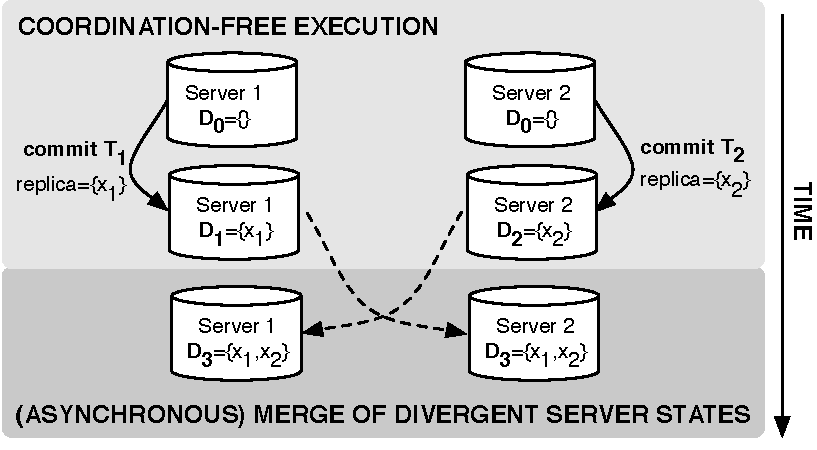
\includegraphics[width=\figscale\columnwidth]{figs/replicas.pdf}\vspace{.5em}
\caption{An example coordination-free execution of two transactions,
  $T_1$ and $T_2$, on two servers. Each transaction writes to its
  local replica, then, after commit, the servers asynchronously
  exchange state and converge to a common state ($D_3$).}
\label{fig:replicas}
\end{figure}

\minihead{Convergence} Transactional availability allows replicas to
maintain valid state \textit{independently}, but it is vacuously
possible to maintain ``consistent'' database states by letting
replicas diverge (contain different state) forever. This guarantees
safety but not liveness~\cite{schneider-concurrent}. To force state
sharing, we adopt the following definition:

\begin{definition}
  A system is \textit{convergent} iff, for each pair of servers, in
  the absence of new writes to the servers and in the
  absence of indefinite communication delays between the servers,
  the servers eventually contain the same versions for any item
  they both store.
\end{definition}

To capture the process of reconciling divergent states, we use the
previously introduced merge operator: given two divergent server
states, we apply the merge operator to produce convergent state. We
assume the effects of merge are atomically visible: either all effects
of a merge are visible or none are. This assumption is not always
necessary but it simplifies our discussion and, as we later discuss,
is maintainable without coordination~\cite{ramp-sigmod14,hat-vldb}.

Our treatment of convergence uses a pair-wise definition (i.e., each
pair converges)~\cite{cac} rather than a system-wide definition (i.e., all nodes
converge). This is more restrictive than system-wide convergence but
allows us to make guarantees on progress despite partitions
between subsets of the servers. This also precludes the use of protocols such
as background consensus, which can stall indefinitely in the presence
of partitions. Like many of the other decisions in our model, this
too could be relaxed if system-wide convergence is sufficient.

\minihead{Maintaining validity} To make sure that both divergent and
convergent database states are valid and, therefore, that transactions
never observe invalid states, we introduce the following property:

\begin{definition}
A system is \textit{globally $I$-valid} iff all replicas always contain
$I$-valid state.
\end{definition}

\minihead{Coordination} Our system model is missing one final
constraint on coordination between concurrent transaction
execution:

\begin{definition}
  A system provides coordination-free execution for a set of
  transactions $T$ iff the progress of executing each $t\in T$ is only
  dependent on $t$'s replica's state (i.e., the versions of the items
  $t$ reads).
\end{definition}

\noindent That is, in a coordination-free execution, each
transaction's progress towards commit/abort is independent of other
operations (e.g., writes, locking, validations) being performed on
behalf of other transactions. Thus, transaction execution cannot rely
on blocking synchronization or communication with other concurrently
running transactions. This coordination-free execution corresponds to
availability under the asynchronous network model used in
distributed computing~\cite{gilbert-cap}: progress is guaranteed
despite the possibility of indefinite delays between servers.


\minihead{A note on partial replication} We have explicitly considered
a replicated model. This was a natural in allowing us to reason about
distributed and multi-versioned databases. Our model captures both
fully replicated databases, where all data items are located on all
servers, and partially replicated databases, where data items are
located on a proper subset of servers. That is, as long as clients can
access \textit{some} copy of the data items they are looking for, they
are allowed to proceed. This allows us to reason about properties over
the entire set of data items (i.e., the abstraction of a replica is a
copy of the whole database), without having to describe data
placement. The distinction is not relevant from the perspective of
reasoning about coordination requirements: if two operations can
proceed independently, irrespective of any side-effects, timing, or
other information produced (or not) by the other, then the question of
whether the data they operate under is stored on multiple servers or
one server is irrelevant.

To illustrate this point, a coordination-free algorithm designed for a
partially replicated system will trivially execute on a fully
replicated system. A coordination-free algorithm designed for a fully
replicated system can execute on a partially replicated system by
having each client operate over its own independent set of versions
until writes quiesce. The latter is not practical but illustrates our
point. In practice, building efficient algorithms for partitioned
databases is challenging; for example, Chapter~\ref{c.ramp} is devoted
to a suite of algorithms for enforcing a common semantics in
partially-replicated databases.

However, in a partially replicated system implementation, checking
whether an invariant is satisfied over a transaction's logical replica
state prior to transaction commit may require transactions to access
servers containing data that they did not directly mention in their
program text. In effect, each transaction must end with an inline
invariant check over any data it modifies and any data referenced by
invariants over the data it modifies to avoid the transaction
committing a non-$I$-valid state. Thus, in a partially replicated
system, this checking can incur communication overhead (e.g., to
ensure that the opposite end of a foreign key relation is
present)---although not always (e.g., to check for a null value upon
insertion). This cost is fundamental to general-purpose invariant
verification in partially replicated systems and has well-studied
relatives in active database
systems~\cite{aiken-confluence,activedb-book} but is---as a
consequence of our decision not to distinguish fully-replicated and
partially-replicated stores---not transparent in our model.

\minihead{A note on convergence} We have chosen to implement
convergence using anti-entropy~\cite{antientropy,optimistic} via the
merge operator. In our model, servers exchange versions by shipping
the \textit{side effects} of transactions rather than the transactions
themselves. Alternatives, such as shipping closures containing the
transactions~\cite{bayou} are possible but are less common in
practice~\cite{queue,dynamo}. Our goal here is that, under a merge
function like set union, transaction effects are propagated, and
transactions are not ``rewritten'' as in alternative extended
transaction models such as compensating actions
(Chapter~\ref{c.relatedwork}).

\minihead{Alternative Merges} As discussed above, merge need not
necessarily be associative, commutative, and idempotent. For example,
in Bayou~\cite{bayou}, users write arbitrary merge functions (that may
not be commutative, associative, or idempotent) and the server
processes determine a total ordering on merge operations in the
background. As long as there is eventually connectivity between all
servers, Bayou guarantees convergence. Thus, the system is convergent
insofar as all servers replay all relevant merge operations even
though the merges themselves are not. Nevertheless, due to their
practical implementation, we focus on associative, commutative, and
idempotent merges here.

\minihead{By example} Figure~\ref{fig:replicas} illustrates a
coordination-free execution of two transactions $T_1$ and $T_2$ on two
separate, fully-replicated physical servers. Each transaction commits
on its local replica, and the result of each transaction is reflected
in the transaction's local server state. After the transactions have
completed, the servers exchange state and, after applying the merge
operator, converge to the same state. Any transactions executing later on
either server will obtain a replica that includes the effects of both transactions.
